% Note that the a4paper option is mainly intended so that authors in
% countries using A4 can easily print to A4 and see how their papers will
% look in print - the typesetting of the document will not typically be
% affected with changes in paper size (but the bottom and side margins will).
% Use the testflow package mentioned above to verify correct handling of
% both paper sizes by the user's LaTeX system.
%
% Also note that the "draftcls" or "draftclsnofoot", not "draft", option
% should be used if it is desired that the figures are to be displayed in
% draft mode.
%
\documentclass[conference]{IEEEtran}
% Add the compsoc option for Computer Society conferences.
%
% If IEEEtran.cls has not been installed into the LaTeX system files,
% manually specify the path to it like:
% \documentclass[conference]{../sty/IEEEtran}





% Some very useful LaTeX packages include:
% (uncomment the ones you want to load)

\usepackage[french]{babel}
\usepackage[utf8]{inputenc}  
\usepackage[T1]{fontenc}      
\usepackage{amsmath}
\usepackage{amssymb}
\usepackage{dsfont}
\usepackage{graphicx}
\usepackage{float}
\usepackage{stmaryrd}
\usepackage{listings}
\usepackage{color}
\usepackage{amsthm}
\usepackage{algorithm}
\usepackage{algorithmic}
\usepackage{caption}
\usepackage{subcaption}
\usepackage{tikz}
\usetikzlibrary{arrows}
\newtheorem{theorem}{Théorème}
\definecolor{forestgreen}{rgb}{0.13,0.54,0.13}  
% *** MISC UTILITY PACKAGES ***
%
%\usepackage{ifpdf}
% Heiko Oberdiek's ifpdf.sty is very useful if you need conditional
% compilation based on whether the output is pdf or dvi.
% usage:
% \ifpdf
%   % pdf code
% \else
%   % dvi code
% \fi
% The latest version of ifpdf.sty can be obtained from:
% http://www.ctan.org/tex-archive/macros/latex/contrib/oberdiek/
% Also, note that IEEEtran.cls V1.7 and later provides a builtin
% \ifCLASSINFOpdf conditional that works the same way.
% When switching from latex to pdflatex and vice-versa, the compiler may
% have to be run twice to clear warning/error messages.






% *** CITATION PACKAGES ***
%
%\usepackage{cite}
% cite.sty was written by Donald Arseneau
% V1.6 and later of IEEEtran pre-defines the format of the cite.sty package
% \cite{} output to follow that of IEEE. Loading the cite package will
% result in citation numbers being automatically sorted and properly
% "compressed/ranged". e.g., [1], [9], [2], [7], [5], [6] without using
% cite.sty will become [1], [2], [5]--[7], [9] using cite.sty. cite.sty's
% \cite will automatically add leading space, if needed. Use cite.sty's
% noadjust option (cite.sty V3.8 and later) if you want to turn this off.
% cite.sty is already installed on most LaTeX systems. Be sure and use
% version 4.0 (2003-05-27) and later if using hyperref.sty. cite.sty does
% not currently provide for hyperlinked citations.
% The latest version can be obtained at:
% http://www.ctan.org/tex-archive/macros/latex/contrib/cite/
% The documentation is contained in the cite.sty file itself.






% *** GRAPHICS RELATED PACKAGES ***
%
\ifCLASSINFOpdf
   %\usepackage[pdftex]{graphicx}
  % declare the path(s) where your graphic files are
  % \graphicspath{{../pdf/}{../jpeg/}}
  % and their extensions so you won't have to specify these with
  % every instance of \includegraphics
  % \DeclareGraphicsExtensions{.pdf,.jpeg,.png}
\else
  % or other class option (dvipsone, dvipdf, if not using dvips). graphicx
  % will default to the driver specified in the system graphics.cfg if no
  % driver is specified.
  % \usepackage[dvips]{graphicx}
  % declare the path(s) where your graphic files are
  % \graphicspath{{../eps/}}
  % and their extensions so you won't have to specify these with
  % every instance of \includegraphics
  % \DeclareGraphicsExtensions{.eps}
\fi
% graphicx was written by David Carlisle and Sebastian Rahtz. It is
% required if you want graphics, photos, etc. graphicx.sty is already
% installed on most LaTeX systems. The latest version and documentation can
% be obtained at: 
% http://www.ctan.org/tex-archive/macros/latex/required/graphics/
% Another good source of documentation is "Using Imported Graphics in
% LaTeX2e" by Keith Reckdahl which can be found as epslatex.ps or
% epslatex.pdf at: http://www.ctan.org/tex-archive/info/
%
% latex, and pdflatex in dvi mode, support graphics in encapsulated
% postscript (.eps) format. pdflatex in pdf mode supports graphics
% in .pdf, .jpeg, .png and .mps (metapost) formats. Users should ensure
% that all non-photo figures use a vector format (.eps, .pdf, .mps) and
% not a bitmapped formats (.jpeg, .png). IEEE frowns on bitmapped formats
% which can result in "jaggedy"/blurry rendering of lines and letters as
% well as large increases in file sizes.
%
% You can find documentation about the pdfTeX application at:
% http://www.tug.org/applications/pdftex





% *** MATH PACKAGES ***
%
%\usepackage[cmex10]{amsmath}
% A popular package from the American Mathematical Society that provides
% many useful and powerful commands for dealing with mathematics. If using
% it, be sure to load this package with the cmex10 option to ensure that
% only type 1 fonts will utilized at all point sizes. Without this option,
% it is possible that some math symbols, particularly those within
% footnotes, will be rendered in bitmap form which will result in a
% document that can not be IEEE Xplore compliant!
%
% Also, note that the amsmath package sets \interdisplaylinepenalty to 10000
% thus preventing page breaks from occurring within multiline equations. Use:
%\interdisplaylinepenalty=2500
% after loading amsmath to restore such page breaks as IEEEtran.cls normally
% does. amsmath.sty is already installed on most LaTeX systems. The latest
% version and documentation can be obtained at:
% http://www.ctan.org/tex-archive/macros/latex/required/amslatex/math/





% *** SPECIALIZED LIST PACKAGES ***
%
%\usepackage{algorithmic}
% algorithmic.sty was written by Peter Williams and Rogerio Brito.
% This package provides an algorithmic environment fo describing algorithms.
% You can use the algorithmic environment in-text or within a figure
% environment to provide for a floating algorithm. Do NOT use the algorithm
% floating environment provided by algorithm.sty (by the same authors) or
% algorithm2e.sty (by Christophe Fiorio) as IEEE does not use dedicated
% algorithm float types and packages that provide these will not provide
% correct IEEE style captions. The latest version and documentation of
% algorithmic.sty can be obtained at:
% http://www.ctan.org/tex-archive/macros/latex/contrib/algorithms/
% There is also a support site at:
% http://algorithms.berlios.de/index.html
% Also of interest may be the (relatively newer and more customizable)
% algorithmicx.sty package by Szasz Janos:
% http://www.ctan.org/tex-archive/macros/latex/contrib/algorithmicx/




% *** ALIGNMENT PACKAGES ***
%
%\usepackage{array}
% Frank Mittelbach's and David Carlisle's array.sty patches and improves
% the standard LaTeX2e array and tabular environments to provide better
% appearance and additional user controls. As the default LaTeX2e table
% generation code is lacking to the point of almost being broken with
% respect to the quality of the end results, all users are strongly
% advised to use an enhanced (at the very least that provided by array.sty)
% set of table tools. array.sty is already installed on most systems. The
% latest version and documentation can be obtained at:
% http://www.ctan.org/tex-archive/macros/latex/required/tools/


\usepackage{mdwmath}
\usepackage{mdwtab}
% Also highly recommended is Mark Wooding's extremely powerful MDW tools,
% especially mdwmath.sty and mdwtab.sty which are used to format equations
% and tables, respectively. The MDWtools set is already installed on most
% LaTeX systems. The lastest version and documentation is available at:
% http://www.ctan.org/tex-archive/macros/latex/contrib/mdwtools/


% IEEEtran contains the IEEEeqnarray family of commands that can be used to
% generate multiline equations as well as matrices, tables, etc., of high
% quality.


%\usepackage{eqparbox}
% Also of notable interest is Scott Pakin's eqparbox package for creating
% (automatically sized) equal width boxes - aka "natural width parboxes".
% Available at:
% http://www.ctan.org/tex-archive/macros/latex/contrib/eqparbox/





% *** SUBFIGURE PACKAGES ***
%\usepackage[tight,footnotesize]{subfigure}
% subfigure.sty was written by Steven Douglas Cochran. This package makes it
% easy to put subfigures in your figures. e.g., "Figure 1a and 1b". For IEEE
% work, it is a good idea to load it with the tight package option to reduce
% the amount of white space around the subfigures. subfigure.sty is already
% installed on most LaTeX systems. The latest version and documentation can
% be obtained at:
% http://www.ctan.org/tex-archive/obsolete/macros/latex/contrib/subfigure/
% subfigure.sty has been superceeded by subfig.sty.

%\usepackage{subcaption}

%\usepackage[caption=false]{caption}
%\usepackage[font=footnotesize]{subfig}
% subfig.sty, also written by Steven Douglas Cochran, is the modern
% replacement for subfigure.sty. However, subfig.sty requires and
% automatically loads Axel Sommerfeldt's caption.sty which will override
% IEEEtran.cls handling of captions and this will result in nonIEEE style
% figure/table captions. To prevent this problem, be sure and preload
% caption.sty with its "caption=false" package option. This is will preserve
% IEEEtran.cls handing of captions. Version 1.3 (2005/06/28) and later 
% (recommended due to many improvements over 1.2) of subfig.sty supports
% the caption=false option directly:
%\usepackage[caption=false,font=footnotesize]{subfig}
%
% The latest version and documentation can be obtained at:
% http://www.ctan.org/tex-archive/macros/latex/contrib/subfig/
% The latest version and documentation of caption.sty can be obtained at:
% http://www.ctan.org/tex-archive/macros/latex/contrib/caption/




% *** FLOAT PACKAGES ***
%
%\usepackage{fixltx2e}
% fixltx2e, the successor to the earlier fix2col.sty, was written by
% Frank Mittelbach and David Carlisle. This package corrects a few problems
% in the LaTeX2e kernel, the most notable of which is that in current
% LaTeX2e releases, the ordering of single and double column floats is not
% guaranteed to be preserved. Thus, an unpatched LaTeX2e can allow a
% single column figure to be placed prior to an earlier double column
% figure. The latest version and documentation can be found at:
% http://www.ctan.org/tex-archive/macros/latex/base/



%\usepackage{stfloats}
% stfloats.sty was written by Sigitas Tolusis. This package gives LaTeX2e
% the ability to do double column floats at the bottom of the page as well
% as the top. (e.g., "\begin{figure*}[!b]" is not normally possible in
% LaTeX2e). It also provides a command:
%\fnbelowfloat
% to enable the placement of footnotes below bottom floats (the standard
% LaTeX2e kernel puts them above bottom floats). This is an invasive package
% which rewrites many portions of the LaTeX2e float routines. It may not work
% with other packages that modify the LaTeX2e float routines. The latest
% version and documentation can be obtained at:
% http://www.ctan.org/tex-archive/macros/latex/contrib/sttools/
% Documentation is contained in the stfloats.sty comments as well as in the
% presfull.pdf file. Do not use the stfloats baselinefloat ability as IEEE
% does not allow \baselineskip to stretch. Authors submitting work to the
% IEEE should note that IEEE rarely uses double column equations and
% that authors should try to avoid such use. Do not be tempted to use the
% cuted.sty or midfloat.sty packages (also by Sigitas Tolusis) as IEEE does
% not format its papers in such ways.





% *** PDF, URL AND HYPERLINK PACKAGES ***
%
\usepackage{url}
% url.sty was written by Donald Arseneau. It provides better support for
% handling and breaking URLs. url.sty is already installed on most LaTeX
% systems. The latest version can be obtained at:
% http://www.ctan.org/tex-archive/macros/latex/contrib/misc/
% Read the url.sty source comments for usage information. Basically,
% \url{my_url_here}.





% *** Do not adjust lengths that control margins, column widths, etc. ***
% *** Do not use packages that alter fonts (such as pslatex).         ***
% There should be no need to do such things with IEEEtran.cls V1.6 and later.
% (Unless specifically asked to do so by the journal or conference you plan
% to submit to, of course. )


% correct bad hyphenation here
%\hyphenation{op-tical net-works semi-conduc-tor}


\begin{document}
%
% paper title
% can use linebreaks \\ within to get better formatting as desired
\title{Classification de sentiments par réseau de neurones récursif tensoriel }


% author names and affiliations
% use a multiple column layout for up to three different
% affiliations
\author{\IEEEauthorblockN{Thomas Moreau}
\IEEEauthorblockA{Ecole polytechnique \\
thomas.moreau@polytechnique.edu}
\and
\IEEEauthorblockN{Bertrand Rondepierre}
\IEEEauthorblockA{Ecole polytechnique\\
bertrand.rondepierre@polytechnique.edu}}

% conference papers do not typically use \thanks and this command
% is locked out in conference mode. If really needed, such as for
% the acknowledgment of grants, issue a \IEEEoverridecommandlockouts
% after \documentclass

% for over three affiliations, or if they all won't fit within the width
% of the page, use this alternative format:
% 
%\author{\IEEEauthorblockN{Michael Shell\IEEEauthorrefmark{1},
%Homer Simpson\IEEEauthorrefmark{2},
%James Kirk\IEEEauthorrefmark{3}, 
%Montgomery Scott\IEEEauthorrefmark{3} and
%Eldon Tyrell\IEEEauthorrefmark{4}}
%\IEEEauthorblockA{\IEEEauthorrefmark{1}School of Electrical and Computer Engineering\\
%Georgia Institute of Technology,
%Atlanta, Georgia 30332--0250\\ Email: see http://www.michaelshell.org/contact.html}
%\IEEEauthorblockA{\IEEEauthorrefmark{2}Twentieth Century Fox, Springfield, USA\\
%Email: homer@thesimpsons.com}
%\IEEEauthorblockA{\IEEEauthorrefmark{3}Starfleet Academy, San Francisco, California 96678-2391\\
%Telephone: (800) 555--1212, Fax: (888) 555--1212}
%\IEEEauthorblockA{\IEEEauthorrefmark{4}Tyrell Inc., 123 Replicant Street, Los Angeles, California 90210--4321}}




% use for special paper notices
%\IEEEspecialpapernotice{(Rapport)}




% make the title area
\maketitle


\begin{abstract}
Dans ce travail on s'intéresse à une problématique d'analyse de sentiments sur des phrases de taille courte à moyennes. Nous nous basons sur le travail de R. Socher \cite{Socher-etal:2013} dont nous reprenons les grandes lignes en les précisant et en l'accompagnant d'une réimplémentation complète de l'algorithme en Python (ainsi que certaines figures pour la clarté de l'exposé). Les méthodes employées entre dans la catégorie du Deep learning, et en particulier dans la classe des réseaux de neurones récurrents.
\end{abstract}
% IEEEtran.cls defaults to using nonbold math in the Abstract.
% This preserves the distinction between vectors and scalars. However,
% if the conference you are submitting to favors bold math in the abstract,
% then you can use LaTeX's standard command \boldmath at the very start
% of the abstract to achieve this. Many IEEE journals/conferences frown on
% math in the abstract anyway.

% no keywords




% For peer review papers, you can put extra information on the cover
% page as needed:
% \ifCLASSOPTIONpeerreview
% \begin{center} \bfseries EDICS Category: 3-BBND \end{center}
% \fi
%
% For peerreview papers, this IEEEtran command inserts a page break and
% creates the second title. It will be ignored for other modes.
\IEEEpeerreviewmaketitle


%%%%%%%%%% Introduction %%%%%%%%%%%%%
\section{Introduction}
Après avoir été abandonnées dans les années 80 devant le manque de technique d'entrainement efficace, le domaine du deep learning est à nouveau en plein essor depuis 2006 notamment depuis les travaux de G. Hinton et Y. Bengio \cite{Hinton:2006:FLA:1161603.1161605,HintonSalakhutdinov2006b,Bengio2007} qui ont abouti à des technique d'entrainement efficaces. Ce problème d'entrainement des modèle est la raison qui avait freiné le développement des réseaux de neuronnes, et bien qu'étant loin d'être résolu, des progrès majeurs ont été faits. De plus, la combinaison des facteurs : mise au point de techniques d'entrainement effectives, augmentation des capacités de stockage, démultiplication de la puissance de calcul a ainsi permis d'atteindre l'état de l'art sur un large spectre de tâches allant de la reconnaissance d'objet au traitement des langues, et en passant par de nombreux domaines d'intérêt du machine learning. 

\subsection{Idées générales et inspirations du deep learning}
L'idée générale du deep learning est de s'inspirer de la physiologie du cerveau humain pour mimiquer de possible mécanismes d'apprentissage. L'aspect profond vient d'une part de cette idée que le cerveau humain organise les neurones par couches et d'autre part de l'idée que les concepts ne s'apprennent pas en se définissant par de nombreux exemples particuliers mais plutôt en généralisant l'information que chacun des élément apporte.

Ceci est parfaitement illustré par l'exemple en figure \ref{3ex} : bien qu'ayant une expérience limitée en l'occurrence sur des moyens de locomotion, nous sommes parfaitement capable d'inférer le type de chacun des véhicules du haut (scooter et vélo) malgré l'écart qu'ils entretiennent avec le modèle moyen. De plus, bien que le troisième exemple soit tout à fait inconnu et d'un type sujet à controverse, nous sommes parfaitement capable de reconnaître qu'il s'agit d'un véhicule, d'un mélange entre plusieurs classes connues entre le scooter, la voiture, le vélo etc.
\begin{figure}[H]
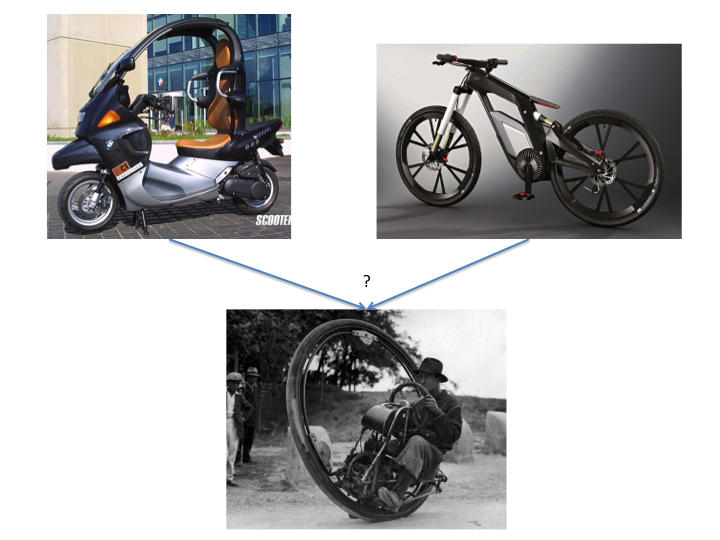
\includegraphics[width=\columnwidth]{fig/Diapositive1.png}
\caption{Trois exemples : en haut de gauche à droite : un scooter et un vélo clairement en marge du modèle moyen. En bas un moyen de locomotion étrange.}
\label{3ex}
\end{figure}

Le processus précédent est rendu possible par notre capacité à généraliser les exemples en concepts. Et c'est exactement la problématique qu'essaie d'aborder le deep learning, où l'aspect profond peut donc également être vu comme cette capacité à généraliser des exemples particuliers par de représentation de plus en plus abstraites suggérant cette idée de couches profondes. Par exemple pour des images ou des objets, on peut imaginer un modèle profond où une première couche constituera les arrêtes visibles au niveau des pixels, puis la seconde celle des parties des objets, puis celle des objets complets, puis les scènes complètes etc... En résumé sur le diagramme suivant : 

\begin{figure}[H]
\centering
\begin{tikzpicture}
\node[draw,rectangle] (Im) at (0,0) {Données};
\node[draw,rectangle] (St) at (2,2) {Concepts abstraits};
\node[draw,rectangle] (Lab) at (4,0) {Labels};

\draw[->] (St) -- (Im);
\draw[->] (St) -- (Lab);
\end{tikzpicture}
\caption{Approche logique}
\end{figure}

\begin{figure}[H]
\centering
\begin{tikzpicture}
\node[draw,rectangle] (Im) at (0,0) {Données};
\node[draw,rectangle] (St) at (2,2) {Concepts abstraits};
\node[draw,rectangle] (Lab) at (4,0) {Labels};

\draw[->] (St) -- (Im);
\draw[->] (Im) -- (Lab);
\end{tikzpicture}
\caption{Approche classique, mais illusoire}
\label{stuff}
\end{figure}

Tout l'enjeu consiste à dire que finalement ce n'est pas vraiment le label qui va être le plus informatif pour construire ces concepts et ces représentations, et qu'il s'agit plus d'une conséquence que d'un identificateur clé. Pour cette raison, l'objectif majeur est d'inverser les transformations que subissent les concepts abstraits pour générer les données sur lesquelles nous travaillons. Une fois que l'on dispose de cela, prendre une décision devient facile.

\subsection{Base du deep learning}
\subsubsection{Le modèle de neurone}
Un neurone peut-être vu comme la plus simple unité computationelle prenant en entrée un signal $x^{input}\in\mathbb{R}^n$, et retournant une sortie $x^{output}$ en combinant d'une part une opération affine et d'autre part un opération non-linéaire $f$:
\begin{align*}
x^{input}&=x \\
x^{output}&=f(Wx^{hidden}+B)
\end{align*}
\begin{figure}[H]
\centering
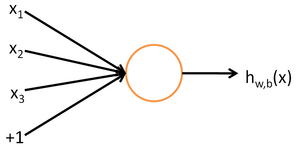
\includegraphics[width=0.75\columnwidth]{fig/SingleNeuron.png}
\caption{Un neurone simple}
\label{Neurone}
\end{figure}
En général la non-linéarité est choisie entre une sigmoïde, une tangente hyperbolique ou encore des fonctions linéaires rectifiées. L'idée est alors de constituer un réseau avec un modèle graphique dans lequel on accumule un grand nombre de neurones répartis dans de (plus ou moins) nombreuses couches.

L'entrainement du modèle se fait alors soit de façon supervisée en ajoutant par exemple une couche de multi-layer perceptron et en optimisant le risque empirique, soit de façon non supervisée en entrainant le réseau comme un modèle génératif sur un critère de type maximum de vraisemblance. Le but est alors d'obtenir une représentation qui permette d'accomplir facilement un certain nombre de tâches, et ici en l'occurrence ce qui nous intéresse est la classification de sentiments.

\subsubsection{Sur la nécessité de la non-linéarité}
Une remarque importante qu'il convient de faire à ce niveau est celle de la présence de la non-linéarité $f$ dans le modèle du neurone. Celle-ci est également une des idées clés du deep learning puisque dans la réalité, l'hypothèse de linéarité n'est certainement pas valables dans les représentations de bas niveau. En revanche c'est bien le cas dans l'espace des concepts dans lequel on essaye de travailler (ce qui n'est bien entendu pas encore réussi) où comme on l'a dit les décisions sont simples : différencier un vélo d'une voiture est très facile. Un modèle linéaire peut donc être parfaitement satisfaisant à condition d'être appliqué dans le bon espace. Cependant une composition de transformations linéaires reste linéaire et il est donc nécessaire d'introduire de la linéarité à un endroit donné. Cette non linéarité sur les représentations de bas niveau est évidente en considérant des exemples où deux objets vont être tout à fait identique du point de vue des concepts, mais avec des formes/textures/couleurs complètement différentes.

\subsubsection{Le théorème d'approximation universelle}
Une des garantie rassurante dans l'emploi de réseaux de neuronnes pour l'apprentissage de fonctions complexes est celle du théorème d'approximation universel (voir par exemple \cite{Hassoun:1995:FAN:526717}). En effet, celui-ci affirme que pour des fonctions d'activation données, un réseau de neuronne est en mesure d'approximer n'importe quelle fonction continue sur un compact. Plus précisément :

\begin{theorem}[Approximation universelle]
Si $f$ est une fonction continue, bornée, strictement croissante, en notant $I_m$ l'hypercube $[0,1]^m$ et $C(I_m)$ les fonctions continues sur $I_m$ alors pour toute fonction $r\in C(I_m)$ et $\varepsilon>0$, il existe $N$ et des constantes $a_i,b_i,w_i$ respectivement dans $\mathbb{R},\mathbb{R},\mathbb{R}^m$ telles que 
$$F(x)=\sum_{i=1}^N a_i f(w_i^T x+b_i)$$
vérifie : $||F-r||_\infty^{I_m}<\varepsilon$. Autrement dit on a densité dans $C(I_m)$.
\end{theorem}

Ce théorème peut-être prouvé toujours valable dans le cas des rectified linear unit avec le max qui n'est plus borné et strictement croissant. La preuve repose sur l'approximation de fonctions convexes par des fonctions affines par morceau et le fait qu'une fonction continue peut s'écrire comme différence de deux fonctions convexes. Voir \cite{2013arXiv1302.4389G}.

En résumé on a espoir de dire qu'il existe effectivement une fonction qui va permettre de mapper les entrées vers une représentation intéressante, et le théorème précédent permet de dire qu'il est effectivement possible d'apprendre ces fonctions avec un réseau de neurones.

Il faut cependant bien noter plusieurs choses : si l'approximation universelle est toujours valable, la question de quelles fonctions peuvent être approximées le plus efficacement avec des architecture de profondeur fixée reste toujours ouverte. En revanche on peut prouver que certaines fonctions représentables facilement avec une architecture de profondeur donnée requièrent avec une architecture de profondeur moindre un nombre de neurone exponentiellement plus grand. Cette idée suggère que la profondeur joue un rôle clef dans l'apprentissage de ces fonctions. 

\subsubsection{Entrainement des réseaux de neurones}
Malgré les garanties théoriques issues de l'approximation universelle ou de la théorie de Vapnik-Chervonenkis, le problème reste d'entrainer effectivement et efficacement les modèles de réseau de neurones. En effet, ceux-ci exhibent des courbures pathologiques qui nécessiteraient l'emploi de méthode du second ordre afin d'être prise en compte, ce qui est malheureusement actuellement trop couteux du fait du nombre de paramètres qui est destiné à être grand.

L'idée est donc de se fixer un critère de type risque empirique ou maximum de vraisemblance selon le cadre dans lequel on se trouve, ce qui se réduit toujours à l'optimisation d'une fonction $E(\theta)$ où $\theta$ est l'ensemble des paramètres du modèle. Le nombre de paramètres étant toujours extrêmement élevé, les méthodes du second ordre impliquant notamment une inversion de la Hessienne sont totalement prohibées. On est alors réduit à toutes les méthodes du premier ordre de type gradient stochastique afin de faire face à des bases de données où le nombre d'exemplaires d'entrainement explose. 


On calcule donc le gradient de $E$ par rapport à ses paramètres. Ce calcul n'est pas toujours simple comme on le verra dans le cas particulier du modèle auquel on s'intéresse pour lequel on explicitera le calcul complet. En effet, du fait de la structure de couche du réseau (et en plus du caractère récurrent dans le cas qui nous intéresse), le calcul du gradient se fait par rétropropagation, c'est à dire que l'erreur se rétropropage du haut du réseau vers le bas. En effet, dans la mesure où les valeurs au nœuds supérieurs sont fonctions de celles aux niveaux inférieurs, on voit bien qu'en dérivant on va devoir propager de haut en bas ces gradients.

Les principes directeurs communément accepté à l'heure actuelle sont les suivants (voir également \cite{DBLP:journals/corr/abs-1206-5533}, ou les dernier travaux du groupe de Yann Le Cun et notamment le dernier article "No more pesky learning rate" : 
\begin{enumerate}
\item Une bonne stratégie d'initialisation des paramètres : c'est le premier progrès réalisé par Hinton en 2006 qui a eu l'idée d'entrainer ses réseaux couche par couche et d'utiliser la sortie pour entrainer la couche suivante. Cette stratégie dite de "greedy layerwise training" permet d'obtenir la plupart du temps une initialisation raisonnable du modèle, qui on l'a constaté est expérimentalement capitale pour obtenir des résultats corrects.
\item Pour stabiliser les méthodes de type gradient stochastique, il est également préférable d'utiliser à chaque itération un ensemble dit mini-batch de quelques exemplaires pour obtenir une estimation moins bruitée du gradient plutôt qu'un seul exemplaire.
\item On utilise alors un algorithme du premier ordre de préférence assez robuste aux valeurs choisies pour les paramètres, typiquement le learning rate dont va grandement dépendre le résultat du modèle. Une méthode à learning rate fixé a peu de chance d'être fructueuse, et il est conseillé d'utiliser des méthodes d'adaptation du learning rate avec les itérations, par exemple RPROP \cite{Riedmiller93adirect}, RMSPROP (Non publié, voir cours de machine learning de Geoff Hinton), AdaGrad \cite{Duchi:2011:ASM:1953048.2021068} ou encore les méthodes de Newton tronquées (ou Hessian-free optimization, voir Mertens et al.\cite{conf/icml/Martens10}).
\item Il est enfin recommandé d'utiliser des architectures qui vont probablement être à la limite de l'overfitting, cependant ici c'est considéré comme une bonne chose, et pour éviter que cela arrive effectivement, on emploie des techniques telles que le dropout (consistant à aléatoirement éteindre des noeuds du réseaux pour éviter la coadaptation des unités), ou encore l'early stopping.
\end{enumerate}

On mentionnera également des méthodes d'accélération de type momentum, gradient accéléré de Nesterov et autres. Ces méthodes sont subtilement reliées les unes aux autres comme l'explique un article non publié de Ilya Sutskever ("On the importance of momentum and initialization in deep learning")expliquant les rapports entre ces méthodes de gradient accéléré et des méthodes de type hessian-free. 

\section{Exposition de la problématique}
Suivant le travail de Richard Socher, nous avons voulu appliquer une technique de deep learning réputée à l'état de l'art sur l'analyse de texte, et plus particulièrement sur l'analyse de sentiments.

\subsubsection{Classification de sentiments}
%Explication des 5 classes et justification
Comme expliqué dans l'article \cite{Socher-etal:2013}, si la classification binaire peut paraître un peu restrictive pour capturer les différentes nuances de langage, un modèle à 5 classes : très négatif, négatif, neutre, positif et très positif permet de capturer la majeure partie de l'information nécessaire afin de classifier les sentiments. Cette observation se fait par rapport à l'annotation de la base de donnée employée (présentée ci-après), où les annotateur disposaient de 7 niveaux de notation des sentiments, et n'utilisaient finalement majoritairement que le neutre et les extrêmes. Ceci a donc poussé à considérer un problème à 5 classes qui capture donc l'essentiel de la variabilité des données.

Ces observations se voient clairement sur la figure de l'article que l'on reprend en figure \ref{Sent}
\begin{figure*}
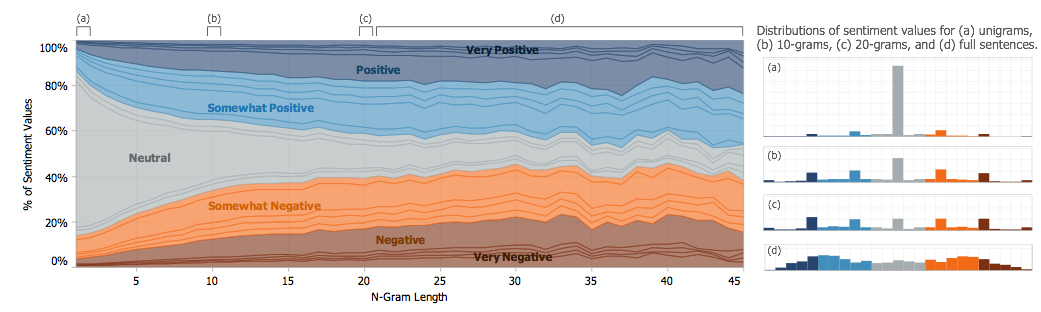
\includegraphics[width=\textwidth]{fig/Sent.png}
\caption{Observation de classification humaine sur la base sentiment treebank}
\label{Sent}
\end{figure*}

L'autre observation qu'il est importante de faire est celle du sentiment ressenti pour les mots seuls : on constate qu'essentiellement les mots sont neutres sauf exception, et les nuances de sentiments apparaissent proportionnellement à la longueur des n-grammes. Ceci explique deux faits :
\begin{itemize}
\item D'une part le succès des approches de type sac de mots sur de longs textes qui permettent de capturer les sentiments par la présence de nombreux mots associés à des sentiments forts, et diluant ainsi les tournures subtiles et négations complètes.
\item D'autre part l'échec de ces mêmes approches pour des phrases plus courtes (Twitter) dans lesquelles le nombre d'occurrences de mots traduisant clairement des sentiments est plus faible, et surtout qui peut être complètement mis en défaut par une négation ou double négation en tête de subordonnée par exemple.
\end{itemize}

On voit donc apparaitre la nécessite de prendre en compte non-seulement le sentiment que traduisent les mots, mais surtout la structure de la phrase, ceci incluant les nuances subtiles telles que les négations. Pour cette raison on s'intéresse à des modèles de réseaux de neurones dits récurent, qui permettent de prendre en compte la structure de la phrase (d'où le terme de récurrence).

\subsubsection{Base de donnée sentiment treebank}
%Présentation de la base avec des schémas.
Pour cette article, Socher et al. ont introduit une nouvelle base de donnée pour les sentiments. Comme expliqué ci-dessus, il s'agit d'une base de données comportant des phrases extraites de critiques de films (rotentomatoes), qui ont été passées dans le parseur de Stanford pour construire un arbre qui représente la phrase et dans lequel chacun des nœuds a été étiqueté avec l'un des 5 labels en fonction du sentiment qu'il représente. On présente deux exemples en figure \ref{trees}.

\begin{figure*}
\begin{subfigure}{0.45\textwidth}
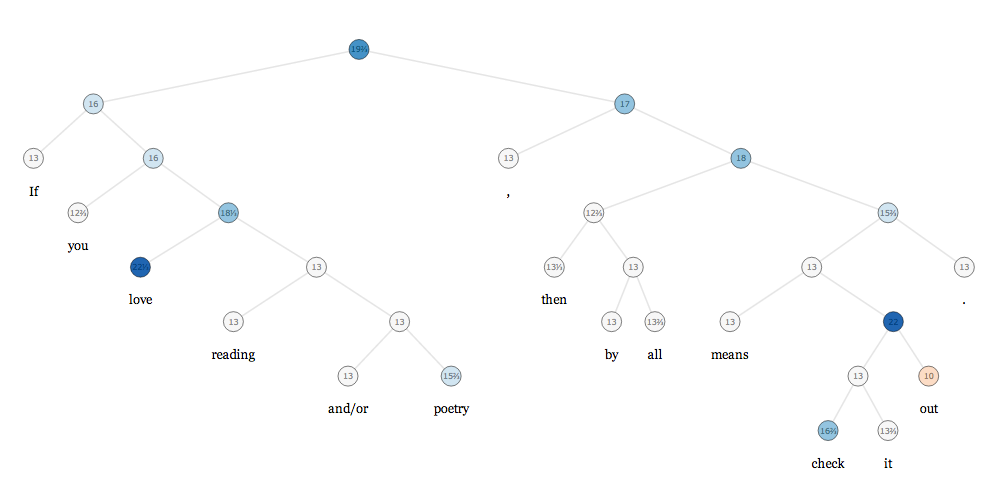
\includegraphics[width=\textwidth]{fig/TB20.png}
\caption{Arbre 20}
\end{subfigure}
\begin{subfigure}{0.45\textwidth}
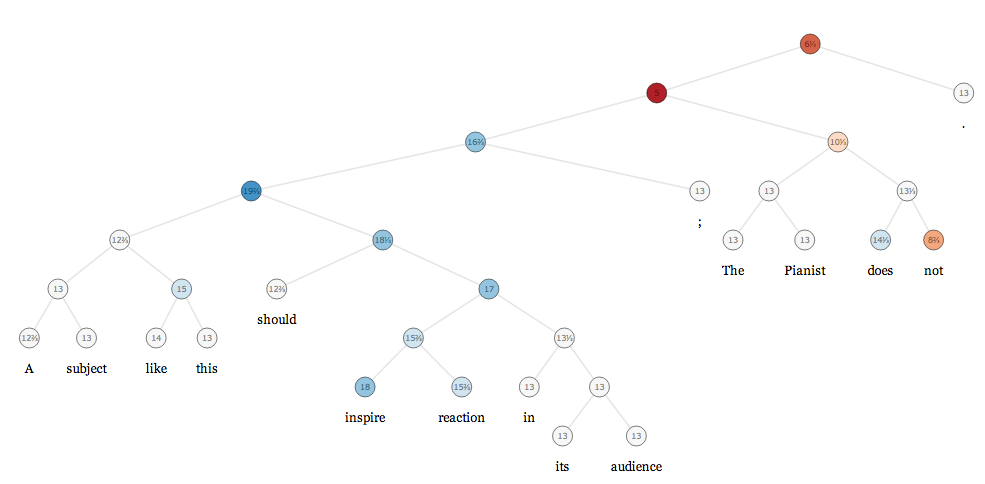
\includegraphics[width=\textwidth]{fig/TB311.png}
\caption{Arbre 311}
\end{subfigure}
\caption{Deux exemple d'arbres parsés et étiquetés.}
\label{trees}
\end{figure*}

Cette base de donnée permet donc bien de prendre en compte les structures et subtilités telles que les négations de proposition comportant des termes positifs qui devient alors à connotation négative. Cela donne également la structure nécessaire à l'application d'un modèle récursif, mais demande donc de modifier quelque peu la structure d'un réseau de neurone pour prendre en compte la structure d'arbre. Nous l'exposons dans ce qui suit.

\section{Modèle de réseau de neurone récursif tensoriel}

Un modèle de réseau de neurones récursif appliqué sur du texte se présente sous la forme de la figure \ref{RNN}.

\begin{figure}
\centering
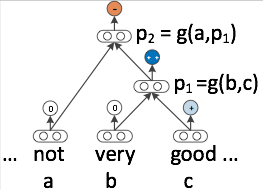
\includegraphics[width=0.75\columnwidth]{fig/RNN.png}
\caption{Schéma des réseaux de neurones récursifs}
\label{RNN}
\end{figure}

Le principe est de construire un arbre à partir de la phrase à analyser, soit à l'aide d'un parseur comme celui de Stanford, soit en utilisant des structures fixes telles qu'un arbre de forme peigne à droite ajoutant un mot à chaque niveau. Bien sûr, pour être efficace, la structure doit prendre en compte la structure de la phrase et il est donc clair qu'utiliser le parseur plutôt qu'une structure fixe conduira à de meilleurs résultats.

Le point commun à tous ces modèles est le suivant : on choisit une représentation pour les mots (par exemple : vecteurs n-dimensionnels ou couples matrices vecteurs). Ensuite pour passer des nœuds disposant d'une représentation (les feuilles à la base qui sont des mots et qui l'ont donc déjà par construction du modèle), on utilise une opération de type neuronale pour construire la représentation des $x^i$ (notation de la figure \ref{RNN}), ie pour le nœud $i$ ayant les enfants $i_1$ et $i_2$ :
$$x^i=g(x^{i_1},x^{i_2})$$
Où l'opération $g$ est à définir en fonction du type de réseau choisi. On détaille ces deux points pour les trois modèles classiques (qui sont ceux présentés dans l'article de Socher)

Ensuite sur chacun des noeuds on ajoute un classifieur de type softmax :
$$x^i\longrightarrow y^i=\frac{exp{\left(W_s x^i_j\right)}}{\sum_{j}exp{\left(W_s x^i_j\right)}}$$
Où $W_s$ est un paramètre du modèle qu'il faudra ajuster conjointement avec autres.

\subsection{Modèles de la littérature}
\subsubsection{Réseau récursif simple}
Dans ce modèle on choisi une représentation d-dimensionnelle pour les mots, et on utilise une opération neuronale non modifiée pour calculer la représentation des nœuds supérieurs à partir de leurs enfants (ici on choisit de travailler sur des digrammes généralisés, cependant le raisonnement est exactement le même si l'on souhaite utiliser des trigrammes ou des modèles plus larges) :

$$x^i=g(x^{i_1},x^{i_2})=f\left(W\begin{bmatrix} x^{i_1} \\ x^{i_2} \end{bmatrix}+b\right)$$
Où $W\in\mathbb{R}^{d\times 2d}$ et $b\in\mathbb{R}^{d}$ et f est la fonction d'activation du réseau. Dans ce modèle, l'essentiel de l'information est contenu dans la matrice $W$ qui va encoder les relations de compositionalité, ce qui n'est cependant pas tout à fait satisfaisant car ne laisse pas énormement de place pour capturer des structures subtiles. Cependant il est suffisamment peu complexe pour être entrainé correctement.

\subsubsection{Réseau récursif vecteur-matrice}
Pour ce modèle, au lieu de choisir une représentation d-dimensionnelle simple, on cherche à encoder les différentes relations de compositionnalité entre les mots dans une matrice associée dans la représentation de chacun d'entre eux. Ainsi les mots sont représentés par couple $(x^i,X^i)$, où $x\in\mathbb{R}^d$, et $X^{i}\in\mathbb{R}^{d\times d}$ et les opérations à effectuer pour passer au niveau suivant sont alors :

$$x^i=g(x^{i_1},x^{i_2})=f\left(W\begin{bmatrix} X^{i_2}x^{i_1} \\ X^{i_1}x^{i_2} \end{bmatrix}+b\right)$$
$$X^i=g_M(X^{i_1},X^{i_2})=f\left(W_M\begin{bmatrix} X^{i_1} \\ X^{i_2} \end{bmatrix}+b_M\right)$$
avec $W,W_M,b,b_M$ à nouveau les paramètres du modèle. Ce modèle a le mérite d'encoder les relation de compositionalité, mais ceci a un coup très élevé : pour chaque mot (le dictionnaire est destiné par nature à être large), il faut avoir un couple dont le nombre total de coefficients est $d+d^2$. Ceci peut rapidement exploser en terme de nombre de paramètre, et surtout en terme d'entrainement cela pose un gros problème car il faut optimiser sur tous ceux-ci, ce qui devient extrêmement difficile à faire efficacement avec des méthodes du premier ordre de type gradient stochastique.

\subsubsection{Réseau récursif tensoriel}
Ce modèle est celui qui a été retenu pour faire les essais puisqu'il allie la simplicité du modèle à une possibilité d'encoder les relations de compositionnalité de façon relativement explicite et ceci pour un coup guère plus élevé que le réseau récursif simple, et beaucoup moins élevé que pour un réseau récursif matrice-vecteur. On choisit donc de même que le simple un représentation des mots dans $\mathbb{R}^d$. La différence majeure se fait dans la fonction $g$ où on ajoute un terme tensoriel censé prendre en compte l'aspect de compositionnalité, conjugué au terme linéaire simple. En bref :

$$x^i=f\left(\begin{bmatrix} x^{i_1} \\ x^{i_2} \end{bmatrix}^T V^{[1:d]}\begin{bmatrix} x^{i_1} \\ x^{i_2} \end{bmatrix} + W\begin{bmatrix} x^{i_1} \\ x^{i_2} \end{bmatrix}\right)$$
Où $W\in\mathbb{R}^{d\times 2d}$, $V$ est un tenseur et pour $h=\begin{bmatrix} x^{i_1} \\ x^{i_2} \end{bmatrix}^T V^{[1:d]}\begin{bmatrix} x^{i_1} \\ x^{i_2} \end{bmatrix}$ on a : $h_j=\begin{bmatrix} x^{i_1} \\ x^{i_2} \end{bmatrix}^T V^{[j]}\begin{bmatrix} x^{i_1} \\ x^{i_2} \end{bmatrix}$, c'est à dire $V\in\mathbb{R}^{d\times 2d\times 2d}$. Il semble que ce modèle permet de trouver un intermédiaire entre un modèle trop simple, et un modèle trop complet difficilement entrainable. On voit dans la partie suivante comment effectuer l'entrainement, et en particulier le calcul des équations de rétropropagation.

\subsubsection{Modèles de sacs de mots}
Enfin, la dernière approche qui n'est pas du deep learning est celle des méthodes dites de sacs de mots consistant à fixer un vocabulaire (éventuellement en le réduisant ou en construisant un dictionnaire plus élaboré qu'un simple comptage), puis construire pour chaque exemplaire à classifier un histogramme des mots de ce vocabulaire présents dans le texte. Après cela, on utilise ces histogramme pour entrainer un classifieur (SVM, Bayésien naïf) utilisé ensuite sur les exemplaires de test. Cette démarche peut également être utilisée exactement de la même manière en augmentant le nombre de mots utilisés simultanément, en choisissant par exemple de travailler sur des bigrammes ou des trigrammes. Cependant comme on peut le voir il s'agit d'une estimation ne reposant ni sur la structure, ni l'ordre des mots présents. L'approche est cependant assez efficace, notamment sur de long textes.

\subsection{Critère d'entrainement}
Dorénavant on s'intéresse exclusivement pour nos développements au réseau de neurone tensoriel récursif, cependant le raisonnement s'applique exactement de la même manière aux autres approches.

En notant $\theta=(W,W_s,V,L)$ les paramètres du modèle (W le terme linéaire, V le tenseur, $W_s$ le paramètre du softmax et enfin $L$ le dictionnaire) on définit l'énergie suivante à partir de la distance de Kullback-Leibler (le signe moins est bien présent contrairement à la formule donnée dans l'article) :
$$E(\theta)=-\sum_{i\in Noeuds}\sum_{j=1}^C t^i_j\log y^i_j+\lambda ||\theta||^2$$
Pour simplifier les notations, on réservera l'index $i$ aux nœuds du réseau.
On peut faire la remarque suivante : le critère d'entrainement est à priori assez mauvais dans la mesure où il va pénaliser exactement de la même manière un label réel très positif qui sera classifié négatif que si il était classifié seulement positif. Le critère ne prend pas du tout en compte la topologie des labels. Dans ce sens il y a une grosse possibilité d'amélioration du modèle.

\subsection{Équations de rétropropogation}
On notera en préliminaire avec le softmax :
$$\sigma_j(y)=\frac{e^{y_j}}{\sum_ k e^{y_k}}$$
que la dérivée est simplement :
$$\partial_i\sigma_j(y)=(\delta_{i,j}-\sigma_i(y))\sigma_j(y)$$

\subsubsection{Gradient par rapport à $W_s$}
On fait donc le calcul de la dérivée par rapport à $[W_s]_{kl}$ qui est différent des suivants puisqu'il ne s'agit pas encore de rétropropagation $y^i_j=\sigma_j(W_s x^i)$ :

\begin{align*}
\frac{\partial E}{\partial [W_s]_{kl}}&=-\sum_{i}\sum_j \frac{t_j^i}{y_j^i} \frac{\partial y_j^i}{\partial [W_s]_{kl}}\\
&=-\sum_i\sum_j \sum_{c=1}^C t_j^i\delta_{kc}(\delta_{cj}-\sigma_c(W_s x^i))x^i_l\\
&=-\sum_i\sum_j t_j^i (\delta_{kj}-y_k^i)x_l^i\\
&= \sum_i (y_k^i -t_k^i) x_l^i
\end{align*}

Donc chaque nœud $i$ contribue au gradient par un terme $(y^i-t^i)(x^i)^T$.

\subsubsection{Gradients par rapport aux autre $\theta$}
Pour comprendre le terme de rétropropagation, on va dériver par rapports aux paramètres autres que $W_s$ :
\begin{align*}
\frac{\partial E}{\partial \theta} &= -\sum_i\sum_j \frac{t_j^i}{y_j^i} \frac{\partial y_j^i}{\partial \theta}\\
&=-\sum_i\sum_j \sum_c t_j^i(\delta_{pj}-y_p^i)\left[W_s\frac{\partial{x^i}}{\partial\theta}\right]_c\\
&= \sum_i\sum_j (y_j^i -t_j^i)\left[W_s\frac{\partial{x^i}}{\partial\theta}\right]_j\\
&=\sum_i (y^i-t^i)W_s\frac{\partial{x^i}}{\partial\theta}
\end{align*}

Pour le nœud $i$ on note $i_g$ et $i_d$ les indices des fils gauche et droite. On a donc :

$$x^i_j=f\left( \begin{bmatrix} x^{i_g} \\ x^{i_d} \end{bmatrix}^T V^{[j]}\begin{bmatrix} x^{i_g} \\ x^{i_d} \end{bmatrix} + W_{j:}\begin{bmatrix} x^{i_g} \\ x^{i_d} \end{bmatrix}\right)$$

On voit donc que $\partial x^i / \partial \theta$ va comporter deux parties : une partie qui constitue le gradient en propre pour le noeud $i$, et une partie en facteur de $\frac{\partial}{\partial\theta}\begin{bmatrix} x^{i_g} \\ x^{i_d} \end{bmatrix}$ qui va se rétropropager aux fils $x^{i_g}$ et $x^{i_d}$.
On note $\delta^{i,s}=W_s^T(y^i-t^i)$. On a alors en considérant que la fonction d'activation a une dérivée simple en fonction d'elle même comme c'est le cas pour $\tanh$ $f'(x)=F(f(x))$

\begin{align*}
\frac{\partial x_j^i}{\partial \theta}&=F(x_j^i) \left( 2\begin{bmatrix} x^{i_g} \\ x^{i_d} \end{bmatrix}^T V^{[j]} +W_{j:}\right)\frac{\partial}{\partial\theta}\begin{bmatrix} x^{i_g} \\ x^{i_d} \end{bmatrix}\\
&+ \begin{bmatrix} x^{i_g} \\ x^{i_d} \end{bmatrix}^T \frac{\partial V^{[j]}}{\partial\theta}\begin{bmatrix} x^{i_g} \\ x^{i_d} \end{bmatrix} + \frac{\partial W_{j:}}{\partial\theta}\begin{bmatrix} x^{i_g} \\ x^{i_d} \end{bmatrix}
\end{align*}

On voit apparaître en première ligne la partie qui se rétropropage aux fils et en deuxième ligne la partie propre au nœud $i$. Ainsi le gradient total va s'écrire :
$$\frac{\partial E}{\partial\theta}=\sum_{i}(\delta^{i,comp})^T \mathcal{E}^{i,\theta}$$
En notant $\mathcal{E}_j^{i,\theta}$ la partie propre au nœud $i$, et $\delta_{j,:}^{i,prop}$ la partie rétropropagée, soit :

$$\mathcal{E}_j^{i,\theta}=\begin{bmatrix} x^{i_g} \\ x^{i_d} \end{bmatrix}^T \frac{\partial V^{[j]}}{\partial\theta}\begin{bmatrix} x^{i_g} \\ x^{i_d} \end{bmatrix} + \frac{\partial W_{j:}}{\partial\theta}\begin{bmatrix} x^{i_g} \\ x^{i_d} \end{bmatrix}$$

$$\delta_{j,:}^{i,prop}=F(x_j^i) \left( 2\begin{bmatrix} x^{i_g} \\ x^{i_d} \end{bmatrix}^T V^{[j]} +W_{j:}\right)$$

Cette dernière partie rétropropagée se somme sur les $j$ pour donner un total :
\begin{align*}
\delta^{i,down}&=\sum_j \delta^{i,comp}_j\delta^{i,prop}_{j:}\\
&=\sum_j 2(\delta_j^{i,comp} F(x^i_j)) V^{[j]}\begin{bmatrix} x^{i_g} \\ x^{i_d} \end{bmatrix}+W^T(\delta^{i,comp}\otimes F(x^i))
\end{align*}

Et on a donc les updates suivants pour calculer les $\delta^{i,comp}$ en notant $p_i$ le père du noeud $i$ qui qualifient l'algorithme de rétropropagation :
\begin{align*}
\delta^{i,comp}&=\delta^{i,s}+\delta^{p_i,down}[1:d] \mbox{ Si i est le fils gauche}\\
&=\delta^{i,s}+\delta^{p_i,down}[d+1:2d] \mbox{ Si i est le fils droit}
\end{align*}

Reste donc à calculer les différentes parties propres pour chaque paramètre.

\subsubsection{Par rapport à W}
La partie propre de la dérivée par rapport à $W_{kl}$ s'écrit :
$$\frac{\partial W_{j:}}{\partial W_{kl}}\begin{bmatrix} x^{i_g} \\ x^{i_d} \end{bmatrix}=\delta_{kj}\begin{bmatrix} x^{i_g} \\ x^{i_d} \end{bmatrix}_l$$

D'où la partie propre (contribution des noeuds pères uniquement) : 
$$\delta^{i,comp}_k \begin{bmatrix} x^{i_g} \\ x^{i_d} \end{bmatrix}_l$$
Soit pour le noeud $i$ une contribution :
$$\frac{\partial E^i}{\partial W}=\delta^{i,comp} \begin{bmatrix} x^{i_g} \\ x^{i_d} \end{bmatrix}^T$$

\subsubsection{Par rapport au tenseur V}
De même la partie propre pour le paramètre $V^{[j]}_{kl}$ :
$$\frac{\partial E^i}{\partial V^{[j]}_{kl}} = \delta_j^{i,comp}\begin{bmatrix} x^{i_g} \\ x^{i_d} \end{bmatrix}_k\begin{bmatrix} x^{i_g} \\ x^{i_d} \end{bmatrix}_l$$

Soit un total :
$$\frac{\partial E^i}{\partial V^{[j]}} = \delta_j^{i,comp}\begin{bmatrix} x^{i_g} \\ x^{i_d} \end{bmatrix}\begin{bmatrix} x^{i_g} \\ x^{i_d} \end{bmatrix}^T$$

\subsubsection{Par rapport au dictionnaire L}
Enfin pour les coefficients de L, seuls les feuilles font une contribution lorsque $x^i=L_k$, qui se lit directement :
$$\frac{\partial E^i}{\partial L_k} = \delta^{i,comp}\delta(x^i=L_k)$$

\section{Résultats expérimentaux}
\subsection{Méthodes d'entrainement retenues}
Dans ce travail, on a voulu considérer deux méthodes d'entrainement : AdaGrad et RMSPROP qui sont deux méthodes online de gradient stochastiques applicables sur des minibatchs qui ont pour essence de réaliser une adaptation du learning rate au cours des itérations.

\subsubsection{AdaGrad}
Défini par Duchi et al. \cite{Duchi:2011:ASM:1953048.2021068}, AdaGrad est un schéma très simple présentant des garanties sous-linéaires dans les borne d'optimisation du regret dans le cas de l'apprentissage par renforcement. Il se résume de la façon suivante : à chaque itération $t$ on calcule le gradient $g_t$, et on stocke la valeur $[a_t]_i=\sum_{t'=1}^t [g_t]_i^2$ et ce pour chacune des composantes $j$ du gradient. On réalise alors l'update suivant :

$$\theta^{t+1}_j=\theta^{t}_j-\frac{\eta}{\sqrt{[a_t]_j}}[g_t]_j$$
Le learning rate $\eta$ a alors une importance que très relative dans la mesure où il va seulement influer sur le poids dans les gradients de la première apparition d'une feature. L'idée derrière cet algorithme est de favoriser les features qui apparaissent rarement mais en étant très informatives par rapport aux features qui apparaissent très souvent sans donner beaucoup d'information. Ces dernières verront donc leur learning rate total beaucoup plus faible que pour les premières. On représente sur les courbes en figure \ref{AdaErreur} la progression de l'erreur avec les itérations.

\begin{figure}[h]
\begin{subfigure}{0.48\columnwidth}
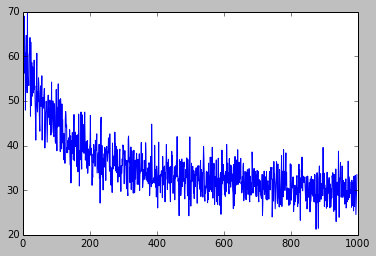
\includegraphics[width=\textwidth]{fig/CourbeMbeAdaGrad.png}
\caption{Erreur sur les mini-batch en fonction des itérations}
\end{subfigure}
\begin{subfigure}{0.48\columnwidth}
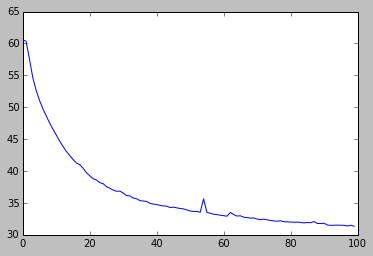
\includegraphics[width=\textwidth]{fig/CourbeValAdaGrad.png}
\caption{Erreur sur le set de validation avec les itérations}
\end{subfigure}
\caption{Erreurs en fonction des itérations pour AdaGrad}
\label{AdaErreur}
\end{figure}

On note sur les courbes (qui sont uniquement des entrainements partiels) que les performance d'AdaGrad sont meilleurs que RPROP et la descente est beaucoup plus rapide à des valeurs intéressantes. C'est donc le mécanisme d'entrainement retenu.

\subsubsection{RPROP et RMSPROP}
RPROP et RMSPROP (Resilient backpropagation et resilient mean square backpropagation) sont deux variantes d'un même algorithme consistant à considérer uniquement le signe des gradients pour effectuer la descente. Le but est d'accélérer de plus en plus l'apprentissage dans les directions qui sont constamment choisies dans le même sens par le gradient, et de ralentir lorsque celui-ci change de signe. 

Plus précisément RPROP se fait par construction sur des batch complets. Après avoir parcouru le training set et évalué le gradient total $g_t$, on effectue l'update $\theta^{t+1}=\theta^t-[\bar{g}_t]_\theta$ sur les paramètres où :

$$
[\bar{g}_t]_\theta=\left\{
\begin{array}{l}
\eta_+[\bar{g}_{t-1}]_\theta \mbox{ Si $[\bar{g}_{t-1}]_\theta$ et $[\bar{g}_{t}]_\theta$ sont de même signe} \\
\eta_-[\bar{g}_{t-1}]_\theta \mbox{ Sinon} 
\end{array}
\right.
$$
Où $\eta_+>1$ et $\eta_-<1$ sont des constantes. Celles-ci traduisent les taux auxquels les vitesses de progression changent.

Le problème avec RPROP est qu'il ne s'applique pas à des versions mini-batch : en effet, l'utilisation du signe implique d'effectuer une opération du type $x/|x|$ sur le gradient total. Afin de réaliser la même chose en minibatch, il faut s'assurer que la constante reste la même sur tous les gradients, ce qui est impossible si celui-ci est recalculé à chaque minibatch. Ainsi, au lieu de diviser par la racine du carré pour obtenir la valeur absolue, on va plutôt conserver en mémoire une trace de la norme précédente, que l'on corrige un peu avec la nouvelle norme calculée. On a alors la variante RMSPROP en divisant par ces carrés moyens :
$$MeanSquare(\theta,t)=(1-\alpha)MeanSquare(\theta,t-1)+\alpha [g_t]_\theta^2$$
Avec habituellement $\alpha<0.5$ et souvent $\alpha=0.1$ (on ne souhaite pas que ce coefficient évolue trop rapidement sur le batch). On conserve la même stratégie d'update en tenant compte de ce point :
$$\theta^{t+1}=\theta^t-[\bar{g}_t]_\theta\frac{[g_t]\theta}{MeanSquare(t,\theta)}$$
Le terme dans la fraction étant censé donner quelque chose de l'ordre du signe du gradient (+1 ou -1 pour les coefficients donc).
Cependant cette technique ne s'est pas montrée extrêmement efficace à l'usage, et a plutôt oscillé entre de mauvaises solutions comme le montre les graphes de la figure \ref{RpropErreur}. Le comportement est représenté sur un millier d'itérations, mais le résultat est le même en allant plus loin on reste sur un plateau en oscillant. La courbe d'erreur avec les mini-batch est erratique du fait du gradient stochastique.

\begin{figure}[h]
\begin{subfigure}{0.48\columnwidth}
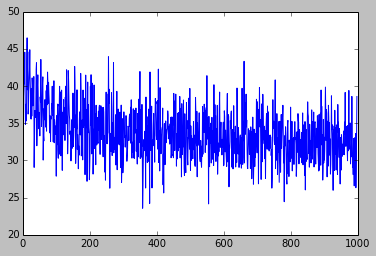
\includegraphics[width=\textwidth]{fig/courbeMbeRprop.png}
\caption{Erreur sur les mini-batch en fonction des itérations}
\end{subfigure}
\begin{subfigure}{0.48\columnwidth}
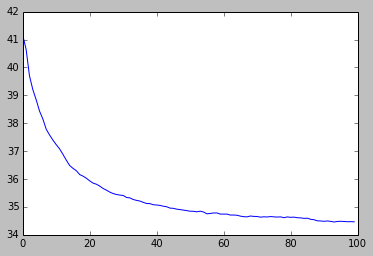
\includegraphics[width=\textwidth]{fig/CourbeValRprop.png}
\caption{Erreur sur le set de validation avec les itérations}
\end{subfigure}
\caption{Erreurs en fonction des itérations}
\label{RpropErreur}
\end{figure}

\subsubsection{Choix des hyperparamètres}
Pour le choix des hyperparamètres, du fait du temps nécessaire à l'entrainement complet d'un réseau de neurones (plusieurs heures avec notre code), nous sommes obligés de fixer un nombre d'itération volontairement trop faible pour obtenir un résultat optimal de l'ordre du millier, puis nous comparons les performances obtenues sur l'ensemble de train et de validation pour juger de la qualité des hyperparamètres utilisés. Pour notre modèle, les hyperparamètres sont : 

\begin{itemize}
\item $\lambda$ pour la régularisation $L^2$.
\item $\eta$ le learning rate de l'AdaGrad.
\item La taille des mini-batchs à chaque itération.
\end{itemize}

Pour cette raison on effectue une recherche des paramètres optimaux sur de grilles de puissances de 10 (du fait du temps nécessaire à l'entrainement). La procédure d'entrainement étant très approchée, il est d'autant moins crucial de choisir des paramètres optimaux avec une grande précision, mais un ordre de grandeur correct est tout à fait suffisant.

\subsubsection{Early stopping}
En emploie une méthode dite $UP_s$ issue de \cite{Prechelt97earlystopping} (Livre "Neural network : a Trick of Trade"). L'idée est de regarder le nombre d'itérations consécutives au cours desquelles l'erreur sur l'ensemble de validation augmente. Cela se résume simplement ainsi \emph{$UP_s$ : si l'erreur de validation augmente sur $s$ itérations consécutives, alors on arrête l'algorithme.}

Le choix de cette méthode a été fait en comparant avec l'erreur de généralisation dite $GL_2$ pour laquelle on arrête l'algorithme lorsque l'erreur de généralisation excède un seuil $\alpha$ donné :
$$GL_\alpha\mbox{ : stop lorsque $100(E_{val}(t)/E_{opt}(t)-1)>\alpha$}$$

Ce dernier critère conduisait cependant à des arrêts beaucoup trop rapides puisque la courbe d'entrainement d'un réseau de neurones est beaucoup moins lisses que celles d'autre techniques.

Nous avons donc choisi un critère d'arrêt $UP_s$ à $s=3$ et une vérification toutes les 100 itérations (le calcul de l'erreur sur l'ensemble de validation rend l'itération beaucoup plus longue que sur un mini-batch, on doit donc le faire seulement à un certain intervalle pour rester rapides).

\subsection{Résultats}
Nous utilisons le même split entre train/validation/test que Richard Socher afin d'être certain de comparer les bons chiffres. Un entrainement complet prend entre 3 et 6 heures avec AdaGrad. Les profils d'entrainement sont ceux en figure \ref{FinErreur} où on voit que l'early stopping a eu lieu juste avant le début de l'overfitting.

\begin{figure}[h]
\begin{subfigure}{0.48\columnwidth}
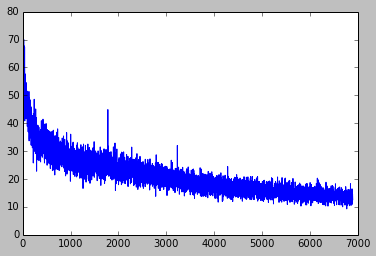
\includegraphics[width=\textwidth]{fig/AdaGradLastTrainMbe.png}
\caption{Erreur sur les mini-batch en fonction des itérations}
\end{subfigure}
\begin{subfigure}{0.48\columnwidth}
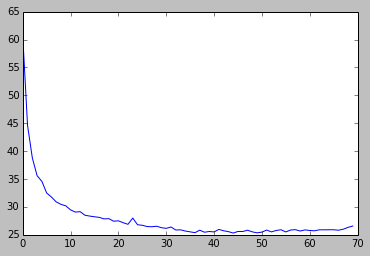
\includegraphics[width=\textwidth]{fig/AdaGradLastTrainVal.png}
\caption{Erreur sur le set de validation avec les itérations}
\end{subfigure}
\caption{Erreurs en fonction des itérations avec AdaGrad}
\label{FinErreur}
\end{figure}

\subsubsection{Problème à 5 classes}
Nous ne sommes à ce jour pas parvenus à reproduire les résultats de l'article de Socher. Le calcul des gradients a été vérifié à de multiple reprise, que ce soit le calcul théorique ou le calcul numérique (comparaison par différences finies). Les valeurs des hyper-paramètres sont dans les range indiqués, la technique d'entrainement est la même, l'architecture du réseau également, et enfin les ensembles train/validation/set sont aussi les mêmes. Pourtant nous sommes toujours en deçà des performances mentionnées dans l'article, et sommes toujours en train d'essayer d'améliorer les résultats. Nous reportons les chiffres suivants à l'heure actuelle :

\begin{center}
\begin{tabular}{|c|c|c|}
\hline
& Tous nœuds & Racines\\ \hline
Résultat 5 classes & 77.83 & 38.28  \\ \hline
Résultat binaire & 66.76 & 66.28 \\ \hline
\end{tabular}
\end{center}

Avec les matrices de confusions pour tous les noeuds mais aussi pour les racines (CM) en figure \ref{CM1}.

\begin{figure}[h]
\begin{subfigure}{0.48\columnwidth}
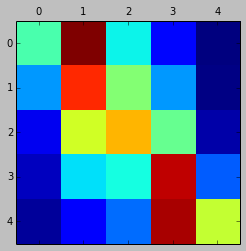
\includegraphics[width=\textwidth]{fig/CMLastTrainRoot.png}
\caption{Racines}
\end{subfigure}
\begin{subfigure}{0.48\columnwidth}
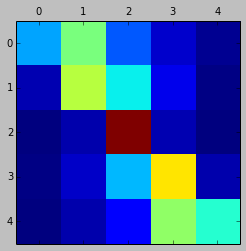
\includegraphics[width=\textwidth]{fig/CMLastTrain.png}
\caption{Nœuds}
\end{subfigure}
\caption{Matrice de confusions noeuds et racine. Les labels sont ordonnées du plus négatif au plus positif.}
\label{CM1}
\end{figure}

Les commentaires à faire sont les suivants : d'une part on constate que malgré le fait que le modèle ne prennent pas du tout en compte la topologie des labels, on arrive cependant à obtenir une classification plutôt correcte en binaire contre toute attente. On constate également que la classification est plus difficile pour les sentiments les plus extrêmes.



\subsubsection{Exemples de phrases}


\section{Conclusion}
Comme cela a déjà été mentionné plus haut, les réseaux de neurones sont un outil extrêmement puissant mais qui demande beaucoup de temps et d'expertise pour être entrainés correctement. Cependant une fois cette phase réussie, ils obtiennent la plupart des temps des résultats à l'état de l'art, en particulier ici sur la classification de sentiments. Ils permettent de formaliser mathématiquement des intuitions simples, et surtout la structure interne du langages.

Le modèle présenté ici représente un très bon compromis dans une catégorie des réseaux qu'il est extrêmement difficile en général d'entrainer , à savoir les réseaux de neurones récursifs. Il allie un modèle simple à un mécanisme de backpropagation efficace du fait de la contrainte forte à partager les mêmes paramètres sur toute la structure. Cependant comme pour toute les méthodes du premier ordre, on est gêné par les courbures pathologiques de la fonction de cout utilisée comme critère, ceci combiné au grand nombre de paramètres à entrainer simultanément.

En revanche, on pourra grandement contester ici le choix qui a été fait de la fonction de coût dans la mesure où on oublie la topologie sur les labels qui est pourtant tout à fait crucial, et un nouveau modèle prenant cet aspect des choses en comptes est à notre avis susceptible de battre le score établi par celui-ci, et notamment en transformant le modèle en un modèle de classification binaire, et non pas en le redéfinissant depuis le départ. En ayant plus d'informations à la base, on devrait parvenir à obtenir un meilleur résultat.
% An example of a floating figure using the graphicx package.
% Note that \label must occur AFTER (or within) \caption.
% For figures, \caption should occur after the \includegraphics.
% Note that IEEEtran v1.7 and later has special internal code that
% is designed to preserve the operation of \label within \caption
% even when the captionsoff option is in effect. However, because
% of issues like this, it may be the safest practice to put all your
% \label just after \caption rather than within \caption{}.
%
% Reminder: the "draftcls" or "draftclsnofoot", not "draft", class
% option should be used if it is desired that the figures are to be
% displayed while in draft mode.
%
%\begin{figure}[H][!t]
%\centering
%\includegraphics[width=2.5in]{myfigure}
% where an .eps filename suffix will be assumed under latex, 
% and a .pdf suffix will be assumed for pdflatex; or what has been declared
% via \DeclareGraphicsExtensions.
%\caption{Simulation Results}
%\label{fig_sim}
%\end{figure}

% Note that IEEE typically puts floats only at the top, even when this
% results in a large percentage of a column being occupied by floats.


% An example of a double column floating figure using two subfigures.
% (The subfig.sty package must be loaded for this to work.)
% The subfigure \label commands are set within each subfloat command, the
% \label for the overall figure must come after \caption.
% \hfil must be used as a separator to get equal spacing.
% The subfigure.sty package works much the same way, except \subfigure is
% used instead of \subfloat.
%
%\begin{figure*}[!t]
%\centerline{\subfloat[Case I]\includegraphics[width=2.5in]{subfigcase1}%
%\label{fig_first_case}}
%\hfil
%\subfloat[Case II]{\includegraphics[width=2.5in]{subfigcase2}%
%\label{fig_second_case}}}
%\caption{Simulation results}
%\label{fig_sim}
%\end{figure*}
%
% Note that often IEEE papers with subfigures do not employ subfigure
% captions (using the optional argument to \subfloat), but instead will
% reference/describe all of them (a), (b), etc., within the main caption.


% An example of a floating table. Note that, for IEEE style tables, the 
% \caption command should come BEFORE the table. Table text will default to
% \footnotesize as IEEE normally uses this smaller font for tables.
% The \label must come after \caption as always.
%
%\begin{table}[!t]
%% increase table row spacing, adjust to taste
%\renewcommand{\arraystretch}{1.3}
% if using array.sty, it might be a good idea to tweak the value of
% \extrarowheight as needed to properly center the text within the cells
%\caption{An Example of a Table}
%\label{table_example}
%\centering
%% Some packages, such as MDW tools, offer better commands for making tables
%% than the plain LaTeX2e tabular which is used here.
%\begin{tabular}{|c||c|}
%\hline
%One & Two\\
%\hline
%Three & Four\\
%\hline
%\end{tabular}
%\end{table}


% Note that IEEE does not put floats in the very first column - or typically
% anywhere on the first page for that matter. Also, in-text middle ("here")
% positioning is not used. Most IEEE journals/conferences use top floats
% exclusively. Note that, LaTeX2e, unlike IEEE journals/conferences, places
% footnotes above bottom floats. This can be corrected via the \fnbelowfloat
% command of the stfloats package.







% conference papers do not normally have an appendix


% use section* for acknowledgement
%\section*{Acknowledgment}
%
%
%The authors would like to thank...





% trigger a \newpage just before the given reference
% number - used to balance the columns on the last page
% adjust value as needed - may need to be readjusted if
% the document is modified later
%\IEEEtriggeratref{8}
% The "triggered" command can be changed if desired:
%\IEEEtriggercmd{\enlargethispage{-5in}}

% references section

% can use a bibliography generated by BibTeX as a .bbl file
% BibTeX documentation can be easily obtained at:
% http://www.ctan.org/tex-archive/biblio/bibtex/contrib/doc/
% The IEEEtran BibTeX style support page is at:
% http://www.michaelshell.org/tex/ieeetran/bibtex/
% argument is your BibTeX string definitions and bibliography database(s)
\bibliography{bibli}{}
\bibliographystyle{IEEEtran}
%
% <OR> manually copy in the resultant .bbl file
% set second argument of \begin to the number of references
% (used to reserve space for the reference number labels box)
%\begin{thebibliography}{1}
%
%\bibitem{IEEEhowto:kopka}
%H.~Kopka and P.~W. Daly, \emph{A Guide to \LaTeX}, 3rd~ed.\hskip 1em plus
% 0.5em minus 0.4em\relax Harlow, England: Addison-Wesley, 1999.
%
%\end{thebibliography}




% that's all folks
\end{document}


